		\paragraph{QuizziPedia::Front-End::Directives::HeaderTextQuestionDirective}
		
		\label{QuizziPedia::Front-End::Directives::HeaderTextQuestionDirective}
		
		\begin{figure}[ht]
			\centering
			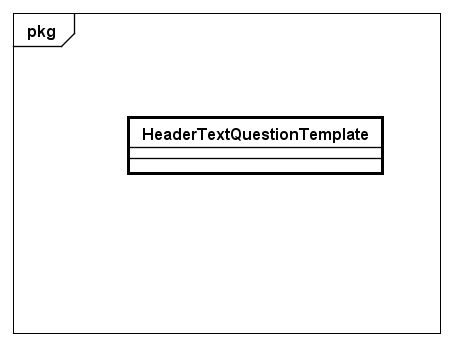
\includegraphics[scale=0.80,keepaspectratio]{UML/Classi/Front-End/QuizziPedia_Front-end_Templates_HeaderTextQuestionTemplate.png}
			\caption{QuizziPedia::Front-End::Directives::HeaderTextQuestionDirective}
		\end{figure} \FloatBarrier
		
		\begin{itemize}
			\item \textbf{Descrizione}: rappresenta il componente grafico che presenta all'utente l'argomento e le parole chiave della domanda che ha a schermo. Viene visualizzato dinamicamente all'interno delle views \texttt{TrainingView} e \texttt{FillingQuestionnaireView} mediante il controller \texttt{QuestionsController};
			\item \textbf{Utilizzo}: viene utilizzato per consentire all'utente la visualizzazione dell'argomento della domanda e le parole chiave associate ad essa;
			\item \textbf{Relazioni con altre classi}: 
			\begin{itemize}
				\item \textbf{IN \texttt{QuestionsModelView}}: classe di tipo modelview la cui istanziazione è contenuta all'interno della variabile di ambiente \$scope di \textit{Angular\ped{G}}. All'interno di essa sono presenti le variabili e i metodi necessari per il \textit{Two-Way Data-Binding\ped{G}} tra le directive che compongono dinamicamente la vista della domanda e il controller \texttt{QuestionsController};
				\item \textbf{OUT \texttt{TrainingView}}: view principale della modalità allenamento. Conterrà i vari templates di ogni domanda dell'allenamento;
				\item \textbf{OUT \texttt{FillingQuestionnaireView}}: view principale per la compilazione del questionario; conterrà i vari templates di ogni domanda appartenente al questionario;   
				\item \textbf{IN \texttt{LangModel}}: rappresenta il modello delle informazioni per la giusta traduzione dell'applicazione.
			\end{itemize}
			\item \textbf{Attributi}:
			\begin{itemize}
				\item \texttt{+ header: Object} \\ Oggetto contenente i campi dati da visualizzare nella direttiva, ovvero:
				\begin{itemize}
					\item \texttt{topic: String} \\ Argomento della domanda;
					\item \texttt{keywords: Array<String>} \\ Parole chiave della domanda.
				\end{itemize}
				\item \texttt{+ controller: String} \\ Stringa contenente il nome del controller della direttiva;
				\item \texttt{+ restrict: String} \\ Stringa che permette di definire le modalità di inserimento della direttiva all'interno della pagina;
				\item \texttt{+ scope: Scope} \\Oggetto \texttt{\$scope} interno della direttiva, contiene le funzionalità per gestire i dati presenti all'interno;
				\item \texttt{+ templateUrl: String} \\ Stringa contenente il percorso del file \textit{HTML\ped{G}} che contiene la direttive.
			\end{itemize}
		\end{itemize}
	